
\chapter{Les évolutions du business modèle des Data Centres}
\label{chap-1}

Ce chapitre a pour but de définir un data centre afin de pouvoir analyser ses problématiques, enjeux et solutions possibles, en vue de comprendre son état actuel et ses limites par rapport aux nouveaux besoins et défis business. Les éléments plus importants de la conception et de l'architecture du data centre seront présentés ainsi que les difficultés qui l'ont amené faire à évoluer son modèle de livraison vers l'approche Cloud Computing.

\section{Data centres et leurs objectifs}

Un data centre (aussi nommé \og ferme de serveurs \fg{}) est un répertoire centralisé pour le stockage, management et distribution de données et informations. Typiquement, un data centre est une installation utilisée pour loger des systèmes informatiques et ses composants associés, tels que systèmes de télécommunication et stockage. 

Les data centres traditionnels hébergent historiquement de nombreuses applications relativement petites ou moyennes, chacune s'exécutant dans une infrastructure matérielle dédiée qui est isolée et protégée des autres systèmes dans la même installation. Ces data centres accueillent du matériel et du logiciel pour multiples unités organisationnelles ou même diverses entreprises. Différents systèmes informatiques au sein d'un tel data centre ont souvent très peu d'éléments en commun en termes de matériel, logiciel ou infrastructure de maintenance, et en général ne communiquent pas entre eux. 


Les tendances de l'informatique vers une approche côté serveur et l'explosion en popularité des services sur internet ont changé ce scénario. Des infrastructures data centre entières ont été dédiées à un seul acteur pour faire fonctionner ses services offerts. Dans ce cadre, un data centre appartient à une seule organisation et utilise des matériels et plateformes logicielles relativement homogènes qui partagent une couche commune de systèmes de management. Ces data centres dédiés exécutent un nombre réduit d'applications (ou services internet) beaucoup plus importants en taille; l'infrastructure commune de management permet alors une meilleure flexibilité de déploiement. 

Ces infrastructures sont montées pour gérer la taille des applications déployées et la haute disponibilité exigée pour ces services, visant en général 99,99\% de durée de fonctionnement (une heure au maximum de temps d'arrêt par an). Il est difficile d'atteindre un fonctionnement libre des failles dans une collection de systèmes matériel et cela devient encore plus complexe avec le grand nombre de serveurs impliqués

\par
Les infrastructures de ces data centres doivent être dimensionnées précisément  en fonction de la charge des applications supportées. Par conséquent, des nouvelles approches ont été proposées pour la construction et l'opération de ces systèmes qui doivent être conçus pour tolérer un nombre important de failles avec très peu ou aucun impact sur la performance et disponibilité des services offerts. \cite{understandingCloudWhatDC}  \cite{datacenterAsComputerIntro}

\section{Organisation d'un data centre et difficultés}

%A data center is generally organized in rows of ‘‘racks” where each rack contains modular assets such as servers, switches, storage ‘‘bricks”, or specialized appliances
Un data centre est en général organisé en lignes de racks où chaque rack contient des dispositifs modulaires tels que serveurs, switches, briques de stockages ou instruments spécialisés. %Trois principaux éléments d'infrastructure constituent les data centres : le stockage, le réseau et l'approvisionnement énergétique.
Des composants essentiels de l'infrastructure, branchés aux racks des data centres d'entreprises tels que compute, stockage et réseau, sont la base sur laquelle les applications business sont construites. Un châssis se présente avec ses propres ventilateurs, source d'alimentation, panier d'interconnexion et module de management. 
Pour réduire l'espace occupé, des serveurs peuvent être compartimentés dans un châssis qui est glissé dans le rack. Un châssis fournit des slots de taille standard où il est possible d'insérer des élément actifs modulaires (aussi connus en tant que \og blades \fg{}). Un seul châssis peut contenir 16 serveurs 1 U; étant donné que les racks supportent 6 châssis, ils ont une capacité théorique de 96 éléments modulaires.


\begin{figure}[h]
\begin{center}
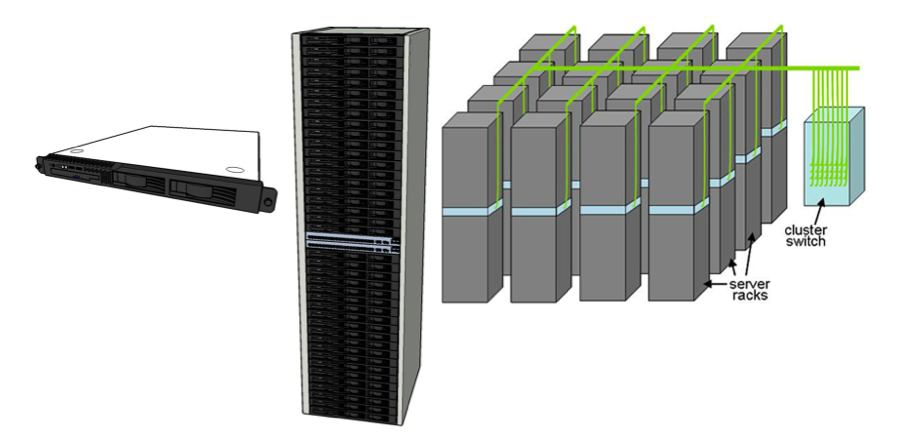
\includegraphics[width=0.7\textwidth]{images/racks} 
\caption{Organisation de racks. \cite{datacenterAsComputerIntro}}\label{racks}
\end{center}
\end{figure}

La figure \ref{racks} montre l'organisation des racks dans un data centre. Un serveur occupe 1 U du rack est montré à gauche. Au milieu on voit un rack et à droite un cluster de racks avec un swtich/routeur de niveau cluster. En général un ensemble de serveurs 1U sont montés dans un rack et inter-connectés avec commutateur Ethernet local. Ces switches au niveau des racks, qui peuvent utiliser des liens de 1 à 10 Gbps, ont un nombre de connexions montantes vers un ou plus switches de niveau cluster (data centre).

Le stockage dans les data centre peut être proposé de diverses manières. Souvent le stockage de haute performance est logé dans des \og  tours de stockage \fg{} qui permettent un accès distant transparent au stockage, indépendamment du nombre et des types des dispositifs de stockage physiques installés. Le stockage peut également être fourni dans une \og  brique de stockage \fg{} plus petite, localisée dans le rack ou slot de châssis ainsi que directement intégrée aux serveurs. Dans tous les cas, un accès réseau efficace au stockage est crucial.

Le problème le plus important dans cette structure est la potentielle insuffisance de bande passante. En général, les connexions montantes sont conçues pour supporter un certain taux de demandes excédentaires puisque la fourniture d'une bande passante entière n'est pas toujours possible. Par exemple, 20 serveurs à 1Gbps chacun doit partager un lien Ethernet montant unique de 10Gps à un taux de demande excédentaire de 2. Cette situation peut être problématique si la charge réseau non locale monte considérablement. Comme le stockage est traditionnellement fourni dans une tour séparée, tout le trafic de stockage traverse le lien montant dans le réseau stockage. Par exemple, l'archivage d'un gros volume peut consommer une importante bande passante. À mesure que les data centres augmentent en taille, une architecture réseau plus extensible devient essentielle.

La consommation d'énergie est également une des préoccupations de la conception des data centres, car les coûts liés sont devenus une part importante de la totalité des coûts pour cette classe de systèmes. Actuellement les CPUs ne sont plus le seul élément cible d'amélioration de l'efficacité énergétique, car ils ne dominent plus la majorité de la consommation. Des problématiques de ventilation et surconsommation d'énergie sont des facteurs de plus en plus critiques dans la conception de data centres.\cite{datacenterAsComputerIntro} \cite{dataCenterEvolution}

\section{Virtualisation et partage de ressources}

Le besoin d'augmenter l'efficacité dans l'utilisation des ressources a conduit à une conception d'infrastructures avec partage de ressources et virtualisation. La virtualisation fait référence à l'abstraction des ressources logiques de leurs couches physiques pour améliorer l'agilité, la flexibilité et la réduction des coûts et ainsi privilégier le business. La virtualisatoin permet de consolider un ensemble de composants d'infrastructures sous-utilisés en un nombre de dispositifs plus petits et mieux utilisés, contribuant à l'économie des coûts.

La virtualisation de serveurs est une méthode pour abstraire le système d'exploitation de la plateforme matérielle. Cela permet aux multiples systèmes d'exploitation ou multiples instances du même système d'exploitation de coexister dans un ou plusieurs processeurs. L'image \ref{virtinfra} illustre le partage de ressources par l'intermédiaire de la virtualisation.

\begin{figure}[h]
\begin{center}
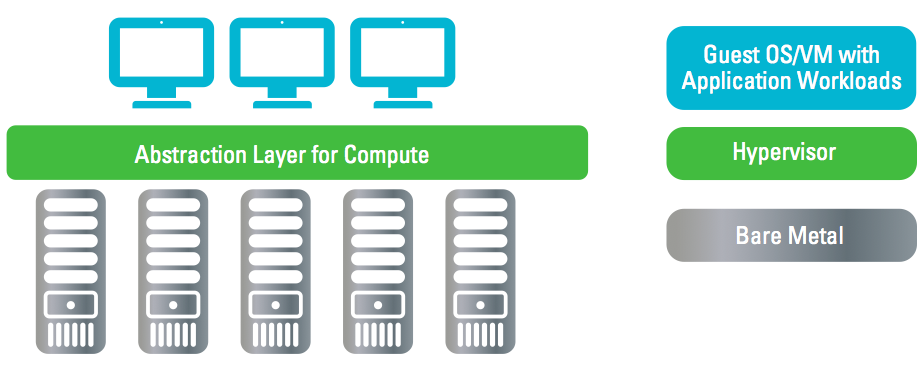
\includegraphics[width=0.98\textwidth]{images/shared_infa_virt} 
\caption{Modèle d'infrastructure à ressources partagées. \cite{journeySDDC}}\label{virtinfra}
\end{center}
\end{figure}

Un hyperviseur ou moniteur de machines virtuelles est inséré entre le système d'exploitation et le matériel pour réaliser la séparation entre le logique et le physique. Les instances de systèmes d'exploitation lancées sont appelées invités, ou systèmes d'exploitation invités. L'hyperviseur fournit l'émulation matérielle aux systèmes invités et gèrent l'allocation de ressources matérielles.  

%Ce modèle apporte des avantages en termes de comment les ressources sont efficacement utilisées avec des charges applicatives idéales.
Ce modèle apporte des avantages pour l'efficacité dans l'utilisation de ressources avec des charges applicatives idéales.
 Cependant, quand une application commence à consommer plus de ressources que l'estimé, il peut arriver des scénarios où les systèmes d'exploitation invités n'ont pas assez de ressources, impactant ainsi la qualité du service business offert. 

Cette approche a apporté une maitrise globale de management, monitoring et outillage. Elle a aussi mis en évidence que le composant \og compute \fg{} de l'infrastructure améliore clairement l'utilisation et automatisation des ressources serveurs. Cette amélioration a été possible grâce à la programmation du contrôle de ressources fournies aux instances invitées. Toutefois, le développement de nouvelles solutions pour gérer la charge dynamique de certaines application faisait toujours défaut. \cite{ibmPlanningVirtCCchap2}\cite{journeySDDC}

%This model has its advantages in terms of how resources are efficiently utilized in ideal applica- tion workloads. However, when one or more appli- cation workloads begin to consume more resourc- es than expected, scenarios could arise where several guest operating systems are short of compute resources, thereby impacting business application service level agreements.
%While this approach brought holistic capacity management, monitoring and tools capabilities, it also provided evidence that infrastructure compute and server resources were truly ben- efiting from improved resource utilization and automation. This was brought about, to a certain extent, by programmatically controlling the resources provided to guest instances. However, new thinking about solutions was still needed to meet the challenges of dynamic workloads of run- the-business applications and compute-intensive enterprise applications.



\section{Le besoin d'un modèle plus dynamique}


Traditionnellement, les data centres d'entreprises sont conçus pour durer pour toujours et atteindre les objectives visibles de l'économie. Cela veut dire que les éléments sous-jacents sont dimensionnés et construits pour supporter le pic de charge projeté en termes de performance, disponibilité et sécurité. Quand la croissance volumétrique projetée ne correspond pas à la réalité, cette méthode de dimensionnement peut conduire à une situation de sous-dimensionnement ou sur-dimensionnement. Ce qui apporte un effet négatif pour les investissements et les effort de réduction de coûts.

En général, pour atteindre une meilleure disponibilité, les infrastructures sont amenées à une sous-utilisation des ressources. Comme la charge des applications varient continuellement dans les applications sur internet, il reste deux choix : soit sous-dimensionner la provision et perdre des clients ou alors sur-dimensionner et gaspiller les ressources. 

Dans tous les cas, un plan détaillé de capacité est fait pour spécifier une série d'investissements importants en matériel et logiciel, dont la capacité est déterminée. L'image suivante illustre cette planification et les situations de problèmes de dimensionnement.


\begin{figure}[h]
\begin{center}
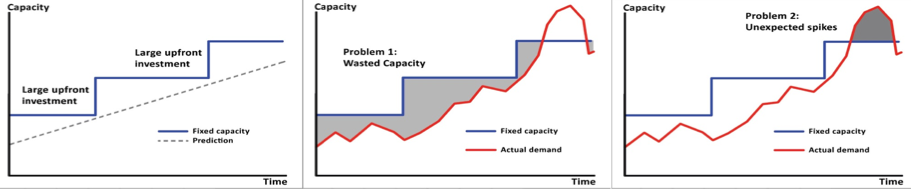
\includegraphics[width=0.98\textwidth]{images/fixed_capacity_load_prediction} 
\caption{Capacité fixe de ressources vs charge prévisionnelle. \cite{awsScaling}}
\end{center}
\end{figure}

Face à cette problématique, un nouveau mode de livraison a été proposé pour aborder les défis du traitement des demandes pour la variation dynamique des charges applicatives. Avec la nouvelle tendance du Cloud Computing et l'infrastructure en tant que service (IaaS), la conception de clusters hautement disponibles et des solutions extensibles peut être architecturée avec des requis non-fonctionnels comme base. 
%With the emergence of the cloud, the new age “mantra” and infrastructure as a service (IaaS) as a delivery model (as illustrated in Figure 3), the challenges of processing demands from dynamic workloads is being addressed. Designing high- availability clusters and scalable solutions can be architected based on nonfunctional requirements.

Avec sa nature extensible, le modèle de livraison cloud permet aux ressources d'être étendues et réduites  dynamiquement en fonction de la consommation. Une couche logicielle d'abstraction, implémentée par les hyperviseurs, virtualise le traitement des ressources physiques,  permettant ainsi au processeur, à la mémoire et aux disques durs de s'accommoder aux variations des demandes. \cite{awsScaling} \cite{journeySDDC}

%One of the biggest technical challenges of running an online business is how well they are able to handle the scalability requirements.  The Load traffic pattern keeps varying for online businesses and accordingly they will have to scale and maintain the acceptable performance levels.  Since the Traffic patterns are fluctuating in online business, they either tend to under provision and loose customers (or) over provision and waste hardware + costs. This problem is well illustrated in the below diagrams.
%Business usually makes detailed capacity planning and large upfront investment in their hardware and software. This HW/SW’s are usually provisioned with fixed capacity.

%Traditionally, enter-prise data centers are designed to last forever and meet visible business objectives, meaning that their underlying components are sized and built for a projected workload. They are also sized and built using application volumetric modeling and nonfunctional requirements such as perfor-mance, availability, scalability and security.

%The infrastructure is designed and provisioned considering the specific volumetric for support- ing the business applications and considering the peak load transaction in jobs per second, avail- ability and scalability requirements. When volu- metric and projected growth do not manifest as envisaged, this method of sizing infrastructure compute and storage could lead to either under- sizing or oversizing the footprint. Often, having such islands of infrastructure compute and storage leads to underutilization of resources. This has a cascading effect on investment and the effort expended toward energy consumption, management overheads, software licenses and data center costs.


%The shortcomings of this model led many enter- prises to the next wave of infrastructure design — utilizing shared infrastructure services and virtualized compute to increase efficiency in resource utilization and ensure that infrastruc- ture is designed and fit for the purpose, and not over-engineered.

%Virtualization refers to the abstraction of logical resources away from their underlying physical resources to improve agility and flexibility, reduce costs, and thus enhance business value. Virtualization allows a set of underutilized physical infrastructure components to be consolidated into a smaller number of better utilized devices, contributing to significant cost savings.

%Server virtualization is a method of abstracting the operating system from the hardware platform. This allows multiple operating systems or multiple instances of the same operating system to coexist on one or more processors. A hypervisor or virtual machine monitor (VMM) is inserted between the operating system and the hardware to achieve this separation. These operating systems are called “guests” or “guest OSs.” The hypervisor provides hardware emulation to the guest operating systems. It also manages allocation of hardware resources between operating systems.

%According to a recent Gartner study, the leading challenges facing today’s data centers are intrinsic to many of the aforementioned business drivers and their associated IT solutions. Top challenges cited include: 
%• Keeping up with data growth 
%• Maintaining system performance and scalability
%• Mitigating network congestion and connectivity issues
%• Minimizing power, cooling and space costs
%• Effectively managing the data center and its infrastructure
%Furthermore, according to a 2011 survey of the Data Center Users’ Group (DCUG), the leading infrastructure challenges included data center availability, high heat densities, energy efficiency and maintaining adequate power densities (see Figure 1). Each of these challenges resonates closely with the leading data center challenges faced by IT professionals.


%\section{Virtualisation}



%Integrated infrastructure solutions are specifically designed to provide advantages compared to a conventional physical infrastructure because they are: 
%•	 Efficient in power usage, space utilization and IT employee productivity
%•	 Economical in initial cost by making use of existing infrastructure and not requiring expensive room upgrades
%•	 Interoperable through simplified design and implementation of systems and components 
%•	 Controllable through planning, monitoring and management over the changing IT environment



%\section{Tendances des meilleures pratiques}


%Integrated infrastructure solutions are specifically designed to provide advantages compared to a conventional physical infrastructure because they are: 
%•	 Efficient in power usage, space utilization and IT employee productivity
%•	 Economical in initial cost by making use of existing infrastructure and not requiring expensive room upgrades
%•	 Interoperable through simplified design and implementation of systems and components 
%•	 Controllable through planning, monitoring and management over the changing IT environment
%\section{Architecture}

%\chapter{Cloud Computing}

% Un regard sur le nouveau \og business model \fg{} apporté par le Cloud Computing, les bénéfices de son adoption et les enjeux pour les infrastructures qui doivent répondre à ce nouveau paradigme, est l'objet de ce chapitre. Il sera démontré pour quelles raisons il nécessaires de faire évoluer les infrastructures actuelles vers le Cloud et pourquoi il n'est pas encore largement adopté.

\section{Cloud Computing}
En termes très simples, le Cloud Computing peut être défini comme un nouveau modèle de consommation et livraison de ressources de \gls{ti} et de services métiers, et est principalement caractérisé par :
\begin{itemize}
\item Libre service à la demande;
\item Service réseau très accessible;
\item Location indépendante de services en commun;
\item Extensibilité et approvisionnement rapides;
\item Paiement à la consommation.
\end{itemize}
%In very simple terms, cloud computing is a new consumption and delivery model for information technology (IT) and business services and is characterized by:
% • On-demand self-service
% • Ubiquitous network access
% • Location-independent resource pooling
% • Rapid elasticity and provisioning
% • Pay-per-use
Les avancements importants dans la virtualisation, réseau, approvisionnement et architectures multi-tenantes ont permis de faire évoluer radicalement les infrastructures de data centres. Le plus grand impact du Cloud Computing vient de l'instauration de nouveaux modèles de consommation et de livraison de services qui supportent l'innovation du business.

%Cloud has evolved from on demand and grid computing, while building on significant advances in virtualization, networking, provisioning, and multitenant architectures. As with any new technology, the exciting impact comes from enabling new service consumption and delivery models that support business model innovation.


L'évolution des data centres a permis de rendre service à une plus grande variété de besoins dans le monde du travail, ce qui implique la prise en compte de plusieurs facteurs lors de la conception face à différents objectifs. Le Cloud Computing est donc né en tant que nouveau paradigme pour les architectures data centre.

%As we have seen, data centers have grown to serve a wide range of business needs, and there are many factors to consider when designing a solution that meets different objectives. Within the past several years, a powerful new paradigm has emerged that has important implications for data center architectures and how they meet these varied objectives. This is the paradigm of cloud computing.

Le Cloud Computing livre dynamiquement des services sur des réseaux à partir d'un ensemble abstrait de ressources. Ces ressources se retrouvent quelque part dans le \og nuage \fg{} (symbole qui fait allusion à la représentation d'internet dans les topologies réseau) disponibles immédiatement à la demande. Les types de ressources ainsi que leur localisation sont transparents aux utilisateurs finaux. Ces utilisateurs se soucient principalement que leurs applications, données et contenus soient sécurisés et disponibles, avec un niveau de qualité spécifié.

%Cloud computing delivers services dynamically over networks from an abstracted set of resources. The resources are somewhere in the cloud and available on demand. The types of resources and their location are transparent to end users. End users primarily care that their applications, data and content are secure and available, with a desired level of quality.

Du point de vue de l'infrastructure, le Cloud Computing fait des fortes demandes aux ressources mutualisées dans une variété de technologies (de compute, de stockage, de réseau) pour leur allocation dynamique. Tout ceci dans un environnement automatisé, orchestré et logiquement diversifié, en conciliant une variété d'applications. L'orchestration permet de mutualiser les ressources à travers multiples data centres pour une réponse dynamique aux besoins clients. 


La virtualisation de serveurs a représentée un premier et important pas à la viabilisation de l'approche Cloud Computing. Toutefois, les autres deux éléments de base de l'infrastructure data centre doivent accompagner ces changements pour qu'on puisse avoir un accès complet aux services offerts par le Cloud. Plus spécifiquement la couche d'abstraction assurée par les hyperviseurs qui ont permis la séparation des systèmes logiques des serveurs physiques dans le cas de la virtualisation de serveurs doit être également appliquée aux matériels réseaux et de stockage. Cela permettra la définition d'un data centre entièrement piloté par du logiciel qui gère les ressources physiques les activant selon la charge applicative spécifiée à assurer.

L'abstraction de ces trois composants matériels est essentielle pour achever le mode de livraison cloud au sein des data centres. La virtualisation des serveurs a déjà atteint son adoption grand public, en 2009 un sondage avait trouvé que 77\% répondant déployait au moins un système virtualisé dans leur data centre \cite{x86ServersVirtualization}. Il se déroule actuellement beaucoup de travail en recherche et développement pour acquérir un niveau équivalent de maturité pour les dispositifs réseau et stockage. 

L'abstraction du stockage signifie la capacité à mutualiser les dispositifs physiques de stockage pour pouvoir les utiliser en tant que volumes de stockage logiques. Cela caractérise la virtulisation du stockage ou le \gls{sds}. Pour l'aspect stockage, il est connu que des solutions \gls{sds} se trouvent disponibles dans le marché, tels que EMC ViPR, HP StoreVirtual, IBM SmartCloud Virtual Storage Center entre autres.

De manière similaire, pour les réseaux il se développe une technologie fournissant une couche d'abstraction pour divers dispositifs réseau pour permettre l'isolation logique et indépendances du matériel. Il se trouve que \gls{sdn} est une des approches proposées pour traiter la problématique de l'abstraction réseau et fait donc l'objet de cette étude. Le chapitre suivant démontrera pour quoi les réseaux traditionnels ne sont pas adaptés aux exigences du Cloud Computing et analysera des exemples sur divers problèmes rencontrés. L'approche SDN et ses apports seront détaillés par la suite.
\cite{ibmPlanningVirtCCchap1}  \cite{cloudReadyJuniperReferenceDef} \cite{journeySDDC}

%From the infrastructure perspective, cloud computing heavily leverages resource pools in a variety of technologies— compute, storage and network—for dynamic allocation in an automated, orchestrated and logically diversified environment, accommodating a variety of applications. Using orchestration, resources can be pooled within and across multiple data centers to provide an environment that responds dynamically to user needs.

%\section{Besoins qui amènent au Cloud}

%Information technology (IT) is at a breaking point, and there is a critical need to improve IT's impact on the business.9
%Consider the following:
% -As much as 85\% of computing capacity sits idle in distributed computing environments.
% -Seventy percent of IT budgets is typically spent on maintaining current IT infrastructures, and only 30\% is typically spent on new capabilities.
% -Over 30\% of consumers notified of a security breach will terminate their relationship with the company that contributed to the breach.
%Clearly, infrastructures need to be more dynamic to free up budgets for new investments and accelerate deployment of superior capabilities being demanded by the business. Nearly all CEOs are adapting business models; cloud adoption can support these changing business dynamics.

%Functional Areas in the Cloud-Ready Data Center
%• Network Infrastructure—provides connectivity and transport for applications and services between users and the data center, within the data center and across multiple data centers. The Network infrastructure has three main sub components, namely the access network, the core network and the edge network.
%• Compute and Storage—represents the compute and storage infrastructure appropriate for applications (rack-mount and chassis-based, cost-effective and multi-core, with unstructured content and highly structured transaction databases). The compute and storage functional area hosts all business applications such as Enterprise Resource Planning (ERP), SaaS, SOA and Web 2.0 applications (among others).
%• Services—supports applications with security, user verification, and entitlement, and application support, including application acceleration, deep packet inspection (DPI), and load balancing
%• Management and Orchestration—ties together all of the elements of the cloud-computing infrastructure, enabling efficient and responsive monitoring, management, and planning

%\section{Nouveau business model}

%Even within the cloud computing space there is a spectrum of offering types. There are five commonly used categories:
%•  Storage as a Service - SaaS Provisioning of database-like services, billed on a utility computing basis, for example, per gigabyte per month.
%•  Infrastructure as a Service - IaaS Provisioning of hardware or virtual computers where the client has control over the OS, therefore allowing the execution of arbitrary software.
%•  Platform as a Service - PaaS Provisioning of hardware and OS, frameworks and databases, for which developers write custom applications. There will be restrictions on the type of software they can write, offset by built-in application scalability.
%•  Software as a Service - SaaS Provisioning of hardware, OS, and special-purpose software made available through the Internet.
%•  Desktop as a Service - DaaS Provisioning of the desktop environment, either within a browser or as a Terminal Server.

%\section{Principaux avantages du Cloud Computing}
%Key benefits of cloud computing:
%• Flexibility – There is the ability to update hardware and software quickly to adhere to customer demands and updates in technology.
%• Savings – There is a reduction of capital expenditures and IT personnel.
%• Location \& Hardware Independence – Users can access application from a web browser connected anywhere on the internet.
%• Multi-tenancy – Resources and cost are shared among many users, allowing overall cost reduction.
%• Reliability – Many cloud providers replicate their server environments in multiply data centers around the globe, which accounts for business continuity and disaster recovery.
%• Scalability – Multiply resources load balance peak load capacity and utilization across multiply hard- ware platforms in different locations
%• Security – Centralization of sensitive data improves security by removing data from the users’ com- puters. Cloud providers also have the staff resources to maintain all the latest security features to help protect data.
%• Maintenance – Centralized applications are much easier to maintain than their distributed counter parts. All updates and changes are made in one centralized server instead of on each user’s computer.


%\section{Barrières au Cloud Computing}

%IT organizations have identified four major barriers to large-scale adoption of cloud services:
%•  Security, particularly data security
%Interestingly, the security concerns in a cloud environment are no different from those in a traditional data center and network. However, since %most of the information exchange between the organization and the cloud service provider is done over the web or a shared network, and %because IT security is handled entirely by an external entity, the overall security risks are perceived as higher for cloud services.
%Some additional factors cited as contributing to this perception:
%– Limited knowledge of the physical location of stored data
%– A belief that multitenant platforms are inherently less secure than single-tenant platforms
%– Use of virtualization as the underlying technology, where virtualization is seen as a relatively new technology
%– Limited capabilities for monitoring access to applications hosted in the cloud
%•  Governance and regulatory compliance
%Large enterprises are still trying to sort out the appropriate data governance model for cloud services, and ensuring data privacy. This is particularly significant when there is a regulatory compliance requirement such as SOX or the European Data Protection Laws.
%•  Service level agreements and quality of service
%Quality of service (availability, reliability, and performance) is still cited as amajor concern for large organizations:
%– Not all cloud service providers have well-defined SLAs, or SLAs that meet stricter corporate standards. Recovery times may be stated as “as soon as possible” rather than a guaranteed number of hours. Corrective measures specified in the cloud provider's SLAs are often fairly minimal and do not cover the potential consequent losses to the client's business in the event of an outage.
%– Inability to influence the SLA contracts. From the cloud service provider's point of view it is impractical to tailor individual SLAs for every client they support.
%– The risk of poor performance is perceived higher for a complex cloud-delivered application than for a relatively simpler on-site service delivery model. Overall performance of a cloud service is dependent on the performance of components outside the direct control of both the client and the cloud service provider, such as the network connection.1. Integrationandinteroperability
I%dentifying and migrating appropriate applications to the cloud is made complicated by the interdependencies typically associated with business applications. Integration and interoperability issues include:
%– A lack of standard interfaces or APIs for integrating legacy applications with cloud services. This is worse if services from multiple vendors are involved.
%– Software dependencies that must also reside in the cloud for performance reasons, but which may not be ready for licensing on the cloud.
%– Interoperability issues between cloud providers. There are worries about how disparate applications on multiple platforms, deployed in geographically dispersed locations, can interact flawlessly and can provide the expected levels of service.